\documentclass[notheorems,9pt]{beamer}

% Packages with options
\usepackage[english]{babel}
\usepackage[mathscr]{euscript}
\usepackage[utf8]{inputenc}

% Primary Packages
\usepackage{amsbsy, amsmath, amssymb, amsthm, bm, blkarray, commath, chngcntr, dsfont, econometrics, gensymb, graphicx, IEEEtrantools, longtable, marginnote, mathrsfs, mathtools, mdframed, natbib, parskip, pgf, setspace, subfigure, tabularx, textcomp, tikz}

% Rest of the setup is in the "setup_beamer" package
\usepackage{setup_beamer}

% Title, Author, Institute
\title{Econ 103: Multiple Linear Regression I}
\author{Manu Navjeevan}
\institute{UCLA}

%%%%%%%%%%%%%%%%%%%%%%%%%%%%%%%%%%%%%%%%%%%%%

\begin{document}
\frame{\titlepage}

\begin{frame}{Content Outline} 
	\label{frame:content-outline}
	\ucla{The Model}:
	\begin{itemize}
		\item Adding more covariates
		\item Assumptions needed for inference
	\end{itemize}
	\ucla{The Estimator}:
	\begin{itemize}
		\item Relation to Single Linear Regression Estimator
		\item Asymptotic Dsitribution
	\end{itemize}
	\ucla{Inference}:
	\begin{itemize}
		\item Hypothesis Tests and Linear Combinations
		\item Confidence Inervals
	\end{itemize}
	\ucla{Modeling Choices}:
	\begin{itemize}
		\item Polynomial Equations, transformations, and interactions
		\item \(R^2\) and goodness of fit
	\end{itemize}
\end{frame}
\section{The Model}

\begin{frame}{The Model: Introduction} 
	\label{frame:model}
	So far we have used the model \(Y = \ucla{\beta_0} + \ucla{\beta_1}X+\eps\) defined by the line of best fit parameters
	\[
		\ucla{\beta_0},\ucla{\beta_1} = \arg\min_{\tilde\beta_0,\tilde\beta_1} \E\left[\left(Y-\tilde\beta_0 - \tilde\beta_1X\right)^2\right]
	.\] 
	to learn about the relationship between a single random variable \(X\) and  \(Y\) and to use  \(X\) to predict  \(Y\).
	\onslide<2->

	\ucla{Examples:}
	\begin{itemize}
		\item Using education to predict income or interpreting the coeffecient \(\ucla{\hat\beta_1}\) to learn about the relationship between the two.
		\item<3-> Learning about the relationship between smoking and heart disease.
	\end{itemize}
\end{frame}
\begin{frame}{The Model: Introduction} 
	\label{frame:model2}
	However, what happens if we have access to multiple explanatory variables \(X_1,\dots,X_p\)?

	\ucla{Examples:}
	\begin{itemize}
		\item Suppose we wanted to impact the joint effect of education \underline{and} experience on age?
		\item Learn about the relationship between smoking, genetic risk, and heart disease
	\end{itemize}
\end{frame}
\begin{frame}{The Model: Introduction} 
	\label{frame:model3}
	As before, we may be interested in the parameters of a ``line of best fit'' between \(Y\) and our explantory variables  \(X_1,\dots,X_p\):
	\[
		\ucla{\beta_0},\ucla{\beta_1},\dots, \ucla{\beta_p} = \arg\min_{b_0,\dots,b_p} \E\left[(Y - b_0 - b_1X_1 - b_2X_2 - \dots - b_pX_p)^2\right]
	.\] 
	\onslide<2->
	Again defining \(\eps = Y - \ucla{\beta_0} - \ucla{\beta_1}X_1 - \dots - \ucla{\beta_p}X_p\) these parameters generate the linear model 
	\[
	    Y = \ucla{\beta_0} + \ucla{\beta_1}X_1 + \dots + \ucla{\beta_p}X_p + \eps
	\]
	where, by the first order conditions for \(\ucla{\beta}\), \(\E[\eps] = \E[\eps X_j] = 0\) for all  \(j = 0,1,\dots,p\). 
\end{frame}
\begin{frame}{The Model: Introduction} 
	\label{frame:model4}
	\ucla{Example 1:} Let \(Y\) be log wages, \(EDU\) be years of college education, and \(EXP\) be years of experience. Prior to this we have estimated the equation
	\begin{equation}
		\label{eq:edu1}
	    Y = \ucla{\beta_0} + \ucla{\beta_1}EDU + \eps
	.\end{equation}
	Now, we will consider estimation and inference on the model
	\begin{equation}
		\label{eq:edu2}
	    Y = \ucla{\beta_0} + \ucla{\beta_1}EDU + \ucla{\beta_2}EXP + \eps
	.\end{equation}
	\onslide<2->
	Note that \(\ucla{\beta_0},\ucla{\beta_1}\) in model \eqref{eq:edu1} will differ from \(\ucla{\beta_0},\ucla{\beta_1}\) in model \eqref{eq:edu2}.
	\begin{itemize}
		\item<3-> In \eqref{eq:edu1} \( \ucla{\beta_0}\) corresponds to the average log wage for someone with no college education
		\item<4-> In \eqref{eq:edu2} \(\ucla{\beta_0}\) will correspond to the average log wage for someone with no college education and no experience
		\item<5-> In \eqref{eq:edu1} \(\ucla{\beta_1}\) corresponds to the expected change in log wage for an additional year of college education
		\item<6-> In \eqref{eq:edu2} \(\ucla{\beta_1}\) corresponds to the expected change in log wage for an additional year of college education \underline{after} controlling for years of experience
 	\end{itemize}
\end{frame}

\begin{frame}{The Model: Introduction} 
	\label{frame:model5}
	\ucla{Example 2:} Let \(Y\) be the (log) final sales price of a home, \(SQFT\) be the square footage of the house, and  \(DAYS\) be the number of days the house has been on the market. Before we estimated and interpreted the linear model:
	\begin{equation}
		\label{eq:house1}
	    Y = \ucla{\beta_0} + \ucla{\beta_1}SQFT + \eps
	.\end{equation} 
	Now, we will consider estimation and inference on the model
	\begin{equation}
		\label{eq:house2}
		Y = \ucla{\beta_0} + \ucla{\beta_1}SQFT + \ucla{\beta_2}DAYS + \eps
	\end{equation}
	\begin{itemize}
		\item<2-> In \eqref{eq:house1} \(\ucla{\beta_0}\) is interpreted as the average log sales price for a home with zero square feet (an empty lot) \underline{regardless} of how long it's been on the market.
		\item<3-> In \eqref{eq:house2} \(\ucla{\beta_0}\) is interpreted as the average log sales price for a home with zero square feet that has just entered the market
		\item<4-> In \eqref{eq:house2} \( \ucla{\beta_1}\) is interpreted as the average change in sales price for a one unit increase in square footage, holding the number of days on the market constant 
	\end{itemize}
\end{frame}
\begin{frame}{The Model: Introduction} 
	\label{frame:intro3}
	\ucla{Example 3:} Finally, let's return to an example from Week 1. Let \(Y\) be a measure of anxiety levels,  \(ENG\) be the number of energy drinks consumed per day, and \(CLS\) be the number of courses being taken. Before we may have estimated the model:
	\begin{equation}
		\label{eq:energy1}
		Y = \ucla{\beta_0} + \ucla{\beta_1}ENG + \eps
	\end{equation}
	Now, we may consider the model
	\begin{equation}
		\label{eq:energy2}
		Y = \ucla{\beta_0} + \ucla{\beta_1}ENG + \ucla{\beta_2}CLS + \eps
	\end{equation}
	\begin{itemize}
		\item<2-3|only@2-3> In \eqref{eq:energy1} we can interpret \(\ucla{\beta_0}\) as the average anxiety level for someone who drinks no energy drinks
		\item<3|only@3> In \eqref{eq:energy2} we can interpret \(\ucla{\beta_0}\) as the average anxiety level for someone who drinks no energy drinks and takes no classes
		\item<4-> In \eqref{eq:energy1} we can interpret \(\ucla{\beta_1}\) as the expected change in anxiety levels for someone who drinks one more energy drink per day
		\item<5-> In \eqref{eq:energy2} we can interpret \(\ucla{\beta_1}\) as the expected change in anxiety levels for an additional energy drink \underline{holding the number of courses being taken constant.}
	\end{itemize}
	\only<6>{
	\red{Question:} How may we expect the signs/magnitutes of the  parameters to change when going from model \eqref{eq:energy1} to model \eqref{eq:energy2}?
 	}	
\end{frame}
\begin{frame}{The Model: Questions}
	\centering
	\red{\Large Questions?}
\end{frame} 
\section{The Estimator}
\begin{frame}{Estimation: Introduction} 
	\label{frame:est1}
	Before, in single linear regression when we were interested in the population line of best fit parameters 
	\[
		\ucla{\beta_0},\ucla{\beta_1} = \arg\min_{b_0,b_1} \E\left[(Y-b_0-b_1X)^2\right],
	\] 
	we estimated them by finding the line of best fit through our sample \(\{Y_i,X_i\}_{i=1}^n\) :
	\[
		\ucla{\hat\beta_0},\ucla{\hat\beta_1} = \arg\min_{b_0,b_1} \frac{1}{n}\sum_{i=1}^n (Y_i - b_0 - b_1X_i)^2
	.\]
	\onslide<2->
	\(\rightarrow\) Have to estimate these parameters using the sample because we don't know the population distribution of  \((Y,X)\)
\end{frame}
\begin{frame}{Estimation: Introduction} 
	\label{frame:est2}
	Now, we are interested in the population line of best fit parameters:
	\[
		\ucla{\beta_0},\ucla{\beta_1}, \dots, \ucla{\beta_p} = \arg\min_{b_0,b_1,\dots,b_p} \E\left[(Y-b_0-b_1X_1-\dots-b_pX_p)^2\right]
	.\]
	\green{Question:} How should we estimate these using our sample \(\{Y_i,X_{1,i},\dots,X_{p,i}\}_{i=1}^n\)?

	\onslide<2->
	Estimate \(\ucla{\beta_0},\dots,\ucla{\beta_p}\) by finding the line of best fit through our sample:
	\[
		\ucla{\hat\beta_0},\ucla{\hat\beta_1},\dots,\ucla{\hat\beta_p} = \arg\min_{b_0,b_1,\dots,b_p} \frac{1}{n}\sum_{i=1}^n (Y_i - b_0 - b_1X_{1,i} - \dots-b_pX_{p,i})^2
	.\] 
\end{frame}
\begin{frame}{Estimation: Introduction} 
	\label{frame:est3}
	Taking first order conditions for \( \ucla{\hat\beta_0},\dots,\ucla{\hat\beta_p}\) above gives us
	\begin{align*}
		\frac{\partial }{\partial b_0}: \frac{1}{n}\sum_{i=1}^n \overbrace{(Y_i - \ucla{\hat\beta_0} - \ucla{\hat\beta_1}X_{1,i} - \dots - \ucla{\hat\beta_p}X_{p,i})}^{\hat\eps_i} &= 0 \\
		\frac{\partial }{\partial b_1}: \frac{1}{n}\sum_{i=1}^n (Y_i - \ucla{\hat\beta_0} - \ucla{\hat\beta_1}X_{1,i} - \dots - \ucla{\hat\beta_p}X_{p,i})X_{1,i} &= 0 \\
		\vdots \\
		\frac{\partial }{\partial b_p}: \frac{1}{n}\sum_{i=1}^n (Y_i - \ucla{\hat\beta_0} - \ucla{\hat\beta_1}X_{1,i} - \dots - \ucla{\hat\beta_p}X_{p,i})X_{p,i} &= 0
	\end{align*}
	\onslide<2->
	This gives us \(p+1\) linear equations to solve for our \(p+1\) parameters. Computers can solve these very quickly, but the explicit formulas for \(\ucla{\hat\beta_0},\ucla{\hat\beta_1},\dots,\ucla{\hat\beta_p}\) become very cumbersome if we don't use linear algebra notation.
\end{frame}
\begin{frame}{Estimation: Aside} 
	\label{frame:est-aside}
	Quickly, it is useful to note the following implication from the first order conditions for \(\ucla{\hat\beta_0},\dots,\ucla{\hat\beta_p}\). Define \(\hat\eps_i = Y_i - \ucla{\hat\beta_0} - \ucla{\hat\beta_1}X_{1,i} - \dots - \ucla{\hat\beta_p}X_{p,i}\). Then 
	\begin{align*}
		\frac{1}{n}\sum_{i=1}^n \hat\eps_i &= 0 \\
		\frac{1}{n}\sum_{i=1}^n \hat\eps_iX_{1,i} &= 0 \\
		\frac{1}{n}\sum_{i=1}^n \hat\eps_iX_{2,i} &= 0 \\
												  &\vdots \\
		\frac{1}{n}\sum_{i=1}^n \hat\eps_iX_{p,i} &= 0
	\end{align*}
\end{frame}
\begin{frame}{Estimation: Asymptotic Distribution} 
	\label{frame:est4}
	Just as in single linear regression, however, the solutions for \( \ucla{\hat\beta_0},\dots,\ucla{\hat\beta_p}\) depend on the data. That is \(\ucla{\hat\beta_0},\dots,\ucla{\hat\beta_p}\) are functions of our sample \(\{Y_i,X_{1,i},\dots,X_{p,i}\}_{i=1}^n\).
	\begin{itemize}
		\item<2-> If we collected a different sample \(\{Y_i,X_{1,i},\dots,X_{2,i}\}_{i=1}^n\), we would get different values for our estimators \( \ucla{\hat\beta_0},\dots,\ucla{\hat\beta_p}\).
	\end{itemize}
	\onslide<3->

	For hypothesis testing we would still like to know the (approximate) distribution of our estimates \( \ucla{\hat\beta_0},\dots,\ucla{\hat\beta_p}\). This will be useful later on as we'd like to calculate objects such as
	\[
		\Pr(|\ucla{\hat\beta_1}| > 5 | \ucla{\beta_1} = -2)
	.\] 
\end{frame}
\begin{frame}{Estimation: Asymptotic Distribution} 
	\label{frame:est5}
	In order for the estimates \(\ucla{\hat\beta_0},\dots,\ucla{\hat\beta_p}\) to have a stable asymptotic distribution and to converge to the true parameters \( \ucla{\beta_0},\dots,\ucla{\beta_p}\), we need to make some (light) assumptions about the underlying distribution of \((Y,X_1,\dots,X_p)\) from which our sample is drawn. 
\end{frame}

\begin{frame}{Estimation: Asymptotic Distribution} 
	\label{frame:est6}
	Assumptions needed for valid inference:
	\begin{itemize}
		\item<1-> \darkucla{Random Sampling}: The data \(\{Y_i,X_{1,i},\dots,X_{p,i}\}\) is independently and identically sampled from the population distribution \((Y,X_1,\dots,X_p)\)
		\begin{itemize}
			\item<1|only@1> Needed to make sure that we are making inferences on the correct population
			\item<2|only@2> \red{Question:} When would this be violated?
		\end{itemize}
		\item<3-> \darkucla{Rank Condition}: The right hand side variables \(X_1,\dots,X_p\) are not linearly dependent, i.e we cannot write
		\[
		    a_1X_1 + a_2X_2 + \dots + a_pX_p = 0
		\]
		for some constants \(a_1,\dots,a_p\) with at least one \(a_k \neq 0\).
		\begin{itemize}
			\item<4|only@4> If this is violated then we can write one random variable as a linear combination of the other ones. 
			\item<5|only@5> To see why this is problematic, suppose that we could write \(X_1 = 2X_2\). Then these two linear models are equivalent
			 \[
				 Y = \ucla{\beta_0} + \ucla{\beta_1}X_1 + \ucla{\beta_2}X_2 + \eps \iff Y = \ucla{\beta_0} + (2\ucla{\beta_1} + \ucla{\beta_2})X_2 + \eps
			.\] 
			The ``line of best fit'' solution is then not unique. We can achieve the same fit by setting the coeffecient on \(X_1\) to be \( \ucla{\ beta_1}\) and the coeffecient on \(X_2\) to be \(\ucla{\beta_2}\) or by setting the coeffecient on \(X_1\) to be zero and the coeffecient on  \(X_2\) to be  \(2\ucla{\beta_1} + \ucla{\beta_2}\).
		\end{itemize}
		\onslide<6->
		\noindent\ucla{\rule{2cm}{0.2mm}}	
		\item<6-> \darkucla{Homoskedasticity}: \(\Var(\eps|X_1= x_1,X_2 = x_2,\dots,X_p = x_p) = \sigma_\eps^2\) for all possible \((x_1,\dots,x_p)\).
		\begin{itemize}
			\item<7|only@7> Like before we can and should relax this. It is not very important to our results but it makes some closed form equations simpler later one.
		\end{itemize}
	\end{itemize}
	\onslide<8->
	And that's it! Really only need \darkucla{Random Sampling} and \darkucla{Rank Condition}.
\end{frame}
\begin{frame}{Estimation: Asymptotic Distribution} 
	\label{frame:asy1}
	Under the assumptions \darkucla{Random Sampling} and \darkucla{Rank Condition} we get the following result for any  \( \ucla{\hat\beta_k}\), \(k = 0,1,\dots,p\).

	Approximately, for large \(n\):
	\[
		\frac{\ucla{\hat\beta_k}-\ucla{\beta_k}}{\hat\sigma_{\beta_k}/\sqrt{n}} \sim N(0,1)\iff \ucla{\hat\beta_k}\sim N\bigg(\ucla{\beta_k}, \underbrace{\sigma_{\beta_k}^2/n}_{=\Var(\ucla{\hat\beta_k})}\bigg)  
	.\]
	\onslide<2->
	\begin{itemize}
		\item<2-> The assumption \darkucla{Homoskedasticity} simply changes the form of  \(\sigma_{\beta_k}^2\) and thus it's estimator  \(\hat\sigma_{\beta_k}^2\). 
		\item<3-> Unlike in single linear regression we will not go over a general form for \(\hat\sigma_{\beta_k}\)
		\begin{itemize}
			\item Typically, all that you need to know is that  \(\hat\sigma_{\beta_k}\) (or the \red{standard error},  \(\hat\sigma_{\beta_k}/\sqrt{n}\) or the \red{variance} \(\hat\sigma_{\beta_k}^2/n\)) will either be given to us directly or found in \(R\) output.
		\end{itemize}
		\item<4->In addition, we will be able to estimate the asymptotic covariance between any two estimates \( \ucla{\hat\beta_j},\ucla{\hat\beta_k}\) for \(j,k = 0,1,\dots,p\).
	\end{itemize}
\end{frame}
\begin{frame}{Estimation: Asymptotic Variance} 
	\label{frame:var-mat}
	To consolidate notation, the variances and covariances are often presented as a \red{Variance-Covariance matrix}. For example, when \(p = 2\) the variance covariance matrix looks like
	\[
		\Cov(\hat\beta) = \begin{pmatrix} \Var(\ucla{\hat\beta_0}) & \Cov(\ucla{\hat\beta_0},\ucla{\hat\beta_1}) & \Cov(\ucla{\hat\beta_0}, \ucla{\hat\beta_2}) \\
		\Cov(\ucla{\hat\beta_1},\ucla{\hat\beta_0}) & \Var(\ucla{\hat\beta_1}) & \Cov(\ucla{\hat\beta_1},\ucla{\hat\beta_2}) \\
		\Cov(\ucla{\hat\beta_2},\ucla{\hat\beta_0}) & \Cov(\ucla{\hat\beta_2},\ucla{\hat\beta_1}) & \Var(\ucla{\hat\beta_2})\end{pmatrix}
	.\] 
	\begin{itemize}
		\item<2-> Note that \(\Cov(X,Y) = \Cov(Y,X)\) so this is a \green{symmetric} matrix 
		\item<3-> Also note that \(\Var(X) = \Cov(X,X)\) which is why we sometimes just call this the \red{Covariance matrix}. 
		\item<4-> In general the \red{Variance-Covariance} matrix will be a \((p+1)\times (p+1)\) matrix (one dimension for each of the slope coefficients and the intercept).
	\end{itemize}
\end{frame}

\begin{frame}{Estimation: Asymptotic Variance} 
	\label{frame:asy3}
	\green{Question:} What influences the asymptotic variance?

	In order to get some intuition for this, we will go over a particular example when \(p = 2\). That is when we want to estimate the model 
	\[
	    Y = \ucla{\beta_0} + \ucla{\beta_1}X_1 + \ucla{\beta_2}X_2 + \eps
	.\]
	\onslide<2->
	In this case, we will be able to get some simple closed form expressions for \(\sigma_{\beta_1}^2\) and  \(\sigma_{\beta_2}^2\).
	\begin{itemize}
		\item<3-> Will provide some insight into what drives the asymptotic variance
	\end{itemize}
\end{frame}

\begin{frame}{Estimation: Asymptotic Variance} 
	\label{frame:asy4}
	Before doing so, let's review the \red{correlation coeffecient}. Recall that for two random variables \(X_1\) and  \(X_2\) the correlation coeffecient  \(\rho_{12}\) is defined
	 \[
		 \rho_{12} = \frac{\Cov(X_1,X_2)}{\sqrt{\Var(X_1)}\sqrt{\Var(X_2)}} 
	.\]
	\onslide<2->
	The correlation coeffecient is a measure of the linear dependence between \(X_1\) and  \(X_2\)
	\begin{itemize}
		\item<2-> If \(\rho_{12} = 1\) then  \(X_1\) and  \(X_2\) are perfectly linearly dependent, that is  \(X_1 = cX_2\) for some constant  \(c\neq 0\)
		\item<3-> If \(\rho_{12} = 0\) then  \(X_1\) and  \(X_2\) are have no linear dependence, that is  \(\Cov(X_1,X_2) = 0\).
	\end{itemize}
\end{frame}

\begin{frame}{Estimation: Asymptotic Variance} 
	\label{frame:asy5}
	With this in mind, the asymptotic variance (under homoskedasticity) \(\hat\sigma_{\beta_1}^2\) for  \(\ucla{\beta_1}\) in the linear model 
	\[
	    Y = \ucla{\beta_0} + \ucla{\beta_1}X_1 + \ucla{\beta_2}X_2 + \eps
	,\] 
	is given
	\[
		\sigma_{\beta_1}^2 = \frac{\sigma_\eps^2}{(1-\rho_{12}^2)\sigma_{X_1}^2} \iff \sqrt{n}(\ucla{\hat\beta_1} - \ucla{\beta_1}) \sim N(0,\sigma_{\beta_1}^2)
	,\] 
	where \(\rho_{12}\) is the correlation coeffecient between  \(X_1\) and  \(X_2\).

	\green{Notice:}
	\begin{itemize}
		\item<2-> As before \(\Var(\hat\beta_1) = \sigma_{\beta_1}^2/n\) is decreasing with \(n\), \(\ucla{\hat\beta_1} \to \ucla{\beta_1}\) as \(n\to\infty\).
		\item<3-> As before \(\sigma_{\beta_1}^2\) is decreasing with \(\sigma_{\eps^2}\) and increasing with  \(\sigma_{X_1}^2\)
		\begin{itemize}
			\item<3|only@3> \(\sigma_\eps^2:\) If points are closer to the line it is easier to make out the line
			\item<3|only@3> \(\sigma_{X_1}^2:\) If points are more spread out, it is easier to make out the line 
		\end{itemize}
		\item<4-> However, now we see that the variance \(\sigma_{\beta_1}^2\) is increasing also as  \(\rho_{12}\uparrow 1\).
		\begin{itemize}
			\item<4|only@4> \red{Intuition:} If \(X_1\) and \(X_2\) are highly correlated, it is difficult to parse out the relationship of  \(X_1\) on  \(Y\) holding \(X_2\) constant. 
		\end{itemize}
	\end{itemize}
\end{frame}
\begin{frame}{Estimation: Asymptotic Variance} 
	\label{frame:estimation}
	To estimate \(\sigma_{\beta_1}^2\) we can estimate each of it's components.
	\[
		\hat\sigma_{\beta_1}^2 = \frac{\hat\sigma_\eps^2}{(1-\hat\rho_{12}^2)\hat\sigma_{X_1}^2} 
	.\] 
	\begin{itemize}
		\item<2-> For \(\hat\sigma_\eps^2\) generate the estimated residuals  \(\hat\eps_i = Y_i - \ucla{\hat\beta_0} - \ucla{\hat\beta_1}X_{1,i} - \ucla{\hat\beta_2}X_{2,i}\) and calculate the sample variance of the estimated residuals:
		\[
			\hat\sigma_\eps^2 = \frac{1}{n}\sum_{i=1}^n \hat\eps_i^2
		.\] 
		\begin{itemize}
			\item Recall that by the first order conditions for \(\ucla{\hat\beta_0}\), \(\frac{1}{n}\sum_{i=1}^n \hat\eps_i = 0\) so that \(\bar{\hat\eps} = 0\)
		\end{itemize}
		\item<3-> For \(\hat\sigma_{X_1}^2\) calculate the sample variance of \(X_1\)
		\[
			\hat\sigma_{X_1}^2 = \frac{1}{n}\sum_{i=1}^n (X_{1,i} - \bar X_1)^2
		.\] 
	\end{itemize}
\end{frame}
\begin{frame}{Estimation: Asymptotic Variance} 
	\label{frame:estimation2}
	To estimate \(\sigma_{\beta_1}^2\) we can estimate each of it's components.
	\[
		\hat\sigma_{\beta_1}^2 = \frac{\hat\sigma_\eps^2}{(1-\hat\rho_{12}^2)\hat\sigma_{X_1}^2} 
	.\]
	\begin{itemize}
		\item To estimate \(\hat\rho_{12}^2\) recall that 
		 \[
			 \rho_{12} = \frac{\Cov(X_1,X_2)}{\sigma_{X_1}\sigma_{X_2}}\implies \hat\rho_{12} = \frac{\widehat\Cov(X_1,X_2)}{\hat\sigma_{X_1}\hat\sigma_{X_2}}  
		.\]
		\begin{itemize}
			\item<2-> We have already covered how to estiamte \(\hat\sigma_{X_1}^2\). Estimating  \(\hat\sigma_{X_2}^2\) follows the same formula
			 \[
				 \hat\sigma_{X_2}^2 = \frac{1}{n}\sum_{i=1}^n (X_{2,i} - \bar X_2)^2
			.\]
			Then, take square roots \(\hat\sigma_{X_1} = \sqrt{\hat\sigma_{X_1}^2}\) and \(\hat\sigma_{X_2} =\sqrt{\hat\sigma_{X_2}^2}\).
			\item<3-> To estimate the covariance note \(\Cov(X_1,X_2) = \E[(X_1 - \mu_{X_1})(X_2 - \mu_{X_2})]\) so 
			\[
				\widehat\Cov(X_1,X_2) = \frac{1}{n}\sum_{i=1}^n (X_{1,i} - \bar X_1)(X_{2,i} - \bar X_2)
			.\] 
		\end{itemize}
	\end{itemize}
\end{frame}

%TODO: Homework question showing that mean residuals is zero
%TODO: Homework question about estiamting the variance

\begin{frame}{Estimation: Asymptotic Variance} 
	\label{frame:asymptotic-variance}
	Let's see an example of this. Suppose we are interested in the joint effect of smoking heavily and drinking heavily on liver failure. 

	That is let \(Y\in \{0,1\}\) denote liver failure, \(X_1 \in \{0,1\}\) denote being a heavy smoker, and \(X_2 \in \{0,1\}\) denote being a heavy drinker and suppose we want to estimate the model 
	\[
	    Y = \ucla{\beta_0} + \ucla{\beta_1}X_1 + \ucla{\beta_2}X_2
	.\]
\end{frame}
\begin{frame}{Estimation: Asymptotic Variance} 
	\label{frame:asymptotic-var}
	After collecting a sample of size \(n= 64\) we estimate  \(\hat\sigma_\eps^2 = 0.25\), \(\hat\sigma_{X_1}^2 = 0.1\), and \(\hat\rho_{12} = 0.5\), where
	\[
	\hat\rho_{12} = \frac{\widehat\Cov(X_1,X_2)}{\hat\sigma_{X_1}\hat\sigma_{X_2}}
	.\] 

	\green{Question:} What is the \underline{standard error} of  \( \ucla{\hat\beta_1}\)?

	\onslide<2->
	\red{Answer:} 
	Recall that the standard error is given \(\hat\sigma_{\beta_1}/\sqrt{n}\). Using the above we get that 
	\[
		\hat\sigma_{\beta_1}^2 = \frac{\hat\sigma_\eps^2}{(1-\hat\rho_{12})\hat\sigma_{X_1}^2} = \frac{0.25}{(1-0.25)0.1} = \frac{10}{3}  
	.\]

	The standard error is then \(\hat\sigma_{\beta_1}/\sqrt{n} = \sqrt{10/3}/\sqrt{64} \approx 0.228\)
\end{frame}
\begin{frame}{Estimation: Asymptotic Variance} 
	\label{frame:var-corr-ex2}
	Now suppose that after collecting a sample of size \(n= 100\) we estimate  \(\hat\sigma_\eps^2 = 0.25\), \(\hat\sigma_{X_1}^2 = 0.1\). This time however, we estimate \(\hat\rho_{12} = 0.75\), where
	\[
		\hat\rho_{12} = \frac{\widehat\Cov(X_1,X_2)}{\hat\sigma_{X_1}\hat\sigma_{X_2}}
	.\] 

	\green{Question:} In this case, what is the standard error  of \(\ucla{\hat\beta_1}\)?

	\onslide<2->
	\red{Answer:} Using the formula above
	\[
		\hat\sigma_{\beta_1}^2 = \frac{\hat\sigma_\eps^2}{(1-\hat\rho_{12})^2\hat\sigma_{X_1}^2} = \frac{0.25}{(1-0.5625)0.1} = \approx 5.714 
	.\] 
	The standard error is then \(\hat\sigma_{\beta_1}/\sqrt{n}\approx \sqrt{5.714}/\sqrt{100} = 0.239\).

	\onslide<3->
	\noindent\ucla{\rule{2cm}{0.2mm}}

	Notice that the standard error is \underline{larger} now than it was when \(n = 64\), despite the fact that our sample size has grown by about 50\%!
\end{frame}

%TODO: Add a homework problem about estimating variance and how it changes with correlation between random variables

\section{Inference}
\begin{frame}{Inference: Introduction} 
	\label{frame:inference-intro}
	Testing single hypothesis about the coeffecients of our regression or linear combinations of coeffecients follows the same procedure.

	If we recall, this procedure consists of constructing a test statistic of the form 
	\[
		t^* = \frac{\text{Estimator} - \text{Null Hypothesis Value}}{\text{Standard Error of Estimator}} 
	,\] 
	and then either computing a p-value or comparing the test statistic directly to a quantile of the standard normal distribution.
\end{frame}

\begin{frame}{Inference: Single Coefficient Testing} 
	\label{frame:inference-single-coeffecient}
	Let's first see how this looks like with a hypothesis test for single coeffecient. Returning to the example from before let \(Y \in \{0,1\}\) be an indicator the existence of liver disease, \(X_1 \in \{0,1\}\) indicate whether or not someone is a heavy smoker, and \(X_2 \in \{0,1\}\) indicate whether someone is a heavy drinker. 

	We want to know if being a heavy smoker is a significant predictor of having liver disease after controlling for whether someone is a heavy drinker. To do so we estimate the following model:
	\[
	    Y = \ucla{\beta_0} + \ucla{\beta_1}X_1 + \ucla{\beta_2}X_2 + \eps
	.\] 
	\onslide<2->
	We want to test the following hypothesis at level \(\alpha = 0.05\):
	\[
		\green{H_0}: \ucla{\beta_1} \leq  0 \vsbox \red{H_1}:\ucla{\beta_1} > 0
	.\]
	\begin{itemize}
		\item<3-> Recall that this essentially amounts to computing the probability that we would observe our estimated value of \(\ucla{\hat\beta_1}\) (or something even further from the null/more positive) if the true value \(\ucla{\beta_1} = 0\).
		\item<4-> Use the result that approximately for large \(n\)
		\[
			\frac{\ucla{\hat\beta_1} - \ucla{\beta_1}}{\hat\sigma_{\beta_1}/\sqrt{n}} \sim N(0,1)
		.\] 
	\end{itemize}
\end{frame}
\begin{frame}{Inference: Single Coefficient Testing} 
	\label{frame:inference}
	Let \(Z \sim N(0,1)\). After collecting a sample of size \(n = 100\) we estimate that  \(\ucla{\hat\beta_1} = 0.04\) and that \(\hat\sigma_{\beta_1}^2 = 4\). Given this we want to compute the \red{p-value}:
	\begin{align*}
		\Pr(\ucla{\hat\beta_1} > 0.03 | \ucla{\beta_1} = 0) &= \Pr(\ucla{\hat\beta_1} - \ucla{\beta_1} > 0.03 - \overbrace{\ucla{\beta_1}}^{=0})\\ &= \Pr\bigg(\frac{\ucla{\hat\beta_1} - \ucla{\beta_1}}{\hat\sigma_{\beta_1}/\sqrt{n}} > \underbrace{\frac{0.03 - 0}{\sqrt{4}/\sqrt{100}}}_{=t^*}  \bigg)\\ 
															&= \Pr(Z > 0.2)\text{\underline{ or, equivalently }}\Pr(Z > t^*) 
	\end{align*}
	and reject the null hypothesis if this probability is less than \(\alpha = 0.05\). 

	\onslide<2->
	Computing this probability using \(R\) we find that  \(p = \Pr(Z > 0.2) \approx 0.42\), since this is larger than \(\alpha = 0.05\) we \green{fail to reject} the null hypothesis.	
\end{frame}
\begin{frame}{Inference: Single Coefficient Testing} 
	\label{frame:inference2}
	As in single linear regression, this is equivalent to checking whether the test statistic \(t^*\) is larger than \(z_{1-\alpha}\) where  \(z_{1-\alpha}\) is such that \(\Pr(Z \leq z_{1-\alpha}) = 1-\alpha\) so that \(\Pr(Z > z_{1-\alpha}) = \alpha\).

	\only<1>{\green{Understanding Check}: Why is checking if \(t^* > z_{1-\alpha}\) equivalent to checking if \(p = \Pr(Z > t^*) < \alpha\)?}
	\onslide<2->
	Since \(\alpha = 0.05\) using the command  {\bf qnorm(0.95)} in \(R\) we find that  \(z_{0.95} = 1.64\). Computing the test statistic as before we find that 
	\[
		t^* = \frac{\ucla{\hat\beta_1} - \text{null hypothesis}}{\hat\sigma_{\beta_1}/\sqrt{n}} = \frac{\ucla{\hat\beta_1} - 0}{\sqrt{4}/\sqrt{100}} = 0.2  
	.\] 
	Since \(t^* =0.2 \leq 1.64 = z_{0.95}\) we \green{fail to reject the null hypothesis} that \(\ucla{\beta_1}\leq 0\). We cannot reject the claim that heavy smoking has no association with having liver disease after controlling for heavy drinking.
\end{frame}
\begin{frame}{Inference: Single Hypothesis Testing} 
	\label{frame:inference3.5}
	We can see that this procedure is exactly the one we considered when we were doing hypothesis tests in single linear regression. In fact we will now go over a general framework for testing  a single null hypothesis of a parameter \(\theta\) whenever we have a result of the form (approximately for large \(n\)):
	\[
		\frac{\hat\theta - \theta}{\hat\sigma_\theta/\sqrt{n}} \sim N(0,1) 
	\]
	where \(\hat\theta\) is an estimator of \(\theta\) and  \(\hat\sigma_\theta/\sqrt{n}\) is the standard error of \(\hat\theta\).

	\ucla{Examples:}
	\begin{itemize}
		\item<2|only@2> By the central limit theorem \[\frac{\bar X-\mu_X}{\hat\sigma_X^2/\sqrt{n}}\sim N(0,1)\]
		\item<3|only@3> For a specific parameter \(\ucla{\beta_k}\) in our multiple linear regression we have that \[\frac{\ucla{\hat\beta_k}-\ucla{\beta_k}}{\hat\sigma_{\beta_k}/\sqrt{n}}\sim N(0,1)\]
		\item<4|only@4> For a linear combination of regression coefficients \(\lambda = a\ucla{\beta_{j}} + b\ucla{\beta_{k}}\) and \(\hat\lambda = a\ucla{\hat\beta_j} + b \ucla{\hat\beta_k}\) we have that \[\frac{\hat\lambda- \lambda}{\hat\sigma_\lambda/\sqrt{n}}\sim N(0,1) .\]
			We will go over how to estimate \(\hat\sigma_\lambda\) using the \red{covariance matrix} shortly.
	\end{itemize}
\end{frame}


\begin{frame}{Inference: Single Hypothesis Testing} 
	\label{frame:inference3}
	As before we have two standard procedure for testing the null hypotheses: \(\green{H_0}: \theta \leq b\), \(\green{H_0}: \theta \geq b\), or \(\green{H_0}: \theta = b\). The first one involves computing p-values:
	\begin{enumerate}
		\item<1|only@1> Compute the test statistic 
		\[
			t^* = \frac{\hat\theta - b}{\hat\sigma_{\theta}/\sqrt{n}}  
		.\] 
		\item<2|only@2> Compute the \underline{p-value}, the probability that we would obtain our observed value of \(\hat\beta\), or something even further from the null hypothesis, if the null hypothesis was correct
		\begin{itemize}
			\item If \(\green{H_0}:\theta = b\) and \(\red{H_1}:\theta\neq b\) compute
			\[
				p = \Pr(|Z| > |t^*|) = 2\Pr(Z > |t^*|)
			.\] 
			\item If \(\green{H_0}:\theta\leq b\) and \(\red{H_1}:\theta> b\) compute
			 \[
				 p = \Pr(Z > t^*)
			.\]
			\item If \(\green{H_0}:\theta\geq b\) and \(\red{H_1}:\theta < b\) compute
			 \[
				 p = \Pr(Z < t^*)
			.\]
		\end{itemize}
		\item<3|only@3> \red{Reject} the null hypothesis in favor of the alternative hypothesis if \(p > \alpha\). Otherwise \green{fail to reject} the null hypothesis.
		\end{enumerate}
\end{frame}

\begin{frame}{Inference: Single Coeffecient Testing} 
	\label{frame:inference4}
		As before this gives us two standard procedure for testing the null hypotheses: \(\green{H_0}: \ucla{\beta_k} \leq b\), \(\green{H_0}: \ucla{\beta_k} \geq b\), or \(\green{H_0}: \ucla{\beta_k} = b\). The second one involves comparing the test statistic to quantiles of the standard normal distribution:
		\begin{enumerate}
		\item<1|only@1> Compute the test statistic or ``t-statistic''
		\[
			t^* = \frac{\ucla{\hat\beta_k} - b}{\hat\sigma_\beta/\sqrt{n}} 
		.\] 
		\item<2|only@2> For a given level \(\alpha\) compute  \(z_{1-\alpha}\) for a one sided alternative or  \(z_{1-\alpha/2}\) for a 2 sided alternative, where \(z_{1-\alpha}\) and  \(z_{1-\alpha/2}\) are such that
		 \[
			 \Pr(Z > z_{1-\alpha}) = \alpha \andbox \Pr(Z > z_{1-\alpha/2}) = \frac{\alpha}{2}
		.\]
		These are called the \(1-\alpha\) and  \(1-\alpha/2\) \red{quantiles} of the standard normal distribution, respectively.
		\begin{itemize}
			\item \(z_{0.9} \approx 1.28 \)
			\item \(z_{0.95} \approx 1.64\)
			\item \(z_{0.975} \approx 1.96\)
			\item \(z_{0.99} \approx 2.32\)
			\item \(z_{0.995} \approx 2.57\)
		\end{itemize}
		\item<3|only@3 > Compare the test statistic \(t^*\) to the quantile  \(z_{1-\alpha}\) or  \(z_{1-\alpha/2}\).
		\begin{itemize}
			\item If \(\green{H_0}: \ucla{\beta_k} = b\) and \(\red{H_1}:\ucla{\beta_k} \neq b\), \red{reject} if \(|t^*| > z_{1-\alpha/2}\)
			\item If \(\green{H_0}: \ucla{\beta_k} \geq b\) and \(\red{H_1}:\ucla{\beta_k} < b\), \red{reject} if  \(t^* < -z_{1-\alpha}\) 
			\item If \(\green{H_0}:\ucla{\beta_k} \leq b\) and \(\red{H_1}:\ucla{\beta_k} > b\), \red{reject} if  \(t^* > z_{1-\alpha}\)
		\end{itemize}
		Otherwise, \green{fail to reject} the null hypothesis.
	\end{enumerate}
\end{frame}

\begin{frame}{Single Hypothesis Testing: Questions}
	\centering
	\red{\Large Questions?}
\end{frame} 

\begin{frame}{Inference: Single Hypothesis Testing} 
	\label{frame:single-hyp-linear-combination}
	Let's see how this works when testing a linear combination of parameters. Returning to our example let \(Y\in \{0,1\}\) denote having liver disease, \(X_1 \in \{0,1\}\) denote being a heavy smoker, and \(X_2 \in \{0,1\}\)  denote being a heavy drinker. We estimate the following linear model
	\[
	    Y = \ucla{\beta_0} + \ucla{\beta_1}X_1 + \ucla{\beta_2}X_2
	.\]
	\onslide<2->
\end{frame}
\begin{frame}{Inference: Single Hypothesis Testing} 
	\label{frame:lincomb2}
	We want to test at level \(\alpha = 0.1\) the null hypothesis that being a heavy smoker or heavy drinker makes you at most 10\% more likely to develop heart disease compared to someone who is neither a heavy smoker nor a heavy drinker. Using our linear model \(Y = \ucla{\beta_0} + \ucla{\beta_1}X_1 + \ucla{\beta_2}X_2\) we approximate
	\begin{align*}
		\;\E[Y | X_1 = 1, X_2 = 1] &= \ucla{\beta_0} + \ucla{\beta_1} + \ucla{\beta_2}  \\
		-\;\E[Y| X_1 = 0, X_2 = 0] &= \ucla{\beta_0}\\
		\rule{3cm}{0.2mm}&\rule{3cm}{0.2mm}\\
		 &= \ucla{\beta_1} + \ucla{\beta_2} 
	\end{align*} 
	\onslide<2-> 
	So, we can state our hypotheses as
	\[
		\green{H_0}: \lambda = \ucla{\beta_1} + \ucla{\beta_2} \leq 0.1 \vsbox \red{H_1}: \lambda = \ucla{\beta_1} + \ucla{\beta_2} > 0.1 
	.\]
	
\end{frame}

\begin{frame}{Inference: Single Hypothesis Testing} 
	\label{frame:lincomb2.5}
	We will aim to test this hypothesis by using the procedure outline above. We will construct \(\hat\lambda = \ucla{\hat\beta_1} + \ucla{\hat\beta_2}\). Because \(\ucla{\hat\beta_1}\) and \(\ucla{\hat\beta_2}\) are both (jointly) approximately normal for large \(n\) we get the following result that
	\[
		\frac{\hat\lambda - \lambda}{\hat\sigma_\lambda/\sqrt{n}} \sim N(0,1) 
	.\]
	where we can calculate \(\hat\sigma_\lambda/\sqrt{n} = \sqrt{\Var(\hat\lambda)}\). We can then use this to do hypothesis testing following the steps above.

	\onslide<2->
	\red{Aside}: I know we have a lot of forms for the variance floating around. To reiterate, basically we use something like \(\sigma_\theta^2\) to say that
	\[
		 \sqrt{n}(\hat\theta - \theta) \sim N(0,\sigma_\theta^2)
	\] 
	then after rearranging this we get that \(\Var(\hat\theta) = \sigma_\theta^2/n\) so that \(\sigma_\theta/\sqrt{n} = \sqrt{\Var(\hat\theta)}\).
\end{frame}
\begin{frame}{Inference: Single Hypothesis Testing} 
	\label{frame:lincomb3}
	After collecting a sample of size \(n= 100\) of  \(\{Y_i,X_{1,i},X_{2,i}\}_{i=1}^{100}\) we find that
	\[
	    \ucla{\hat\beta_0} = 0.05\;\;\ucla{\hat\beta_1} = 0.02\;\;\ucla{\hat\beta_2} = 0.15 \implies \hat\lambda = \ucla{\hat\beta_1}+\ucla{\hat\beta_2} = 0.17
	.\] 
	\only<1>{\green{Question:} How do we interpret \(\hat\lambda\)?}
	\onslide<2->
	We also estimate the following covariance matrix:
	\begin{equation*}
		\Cov(\ucla{\hat\beta}) = 
	  \begin{blockarray}{lccc}
		  & \ucla{\hat\beta_0} & \ucla{\hat\beta_1} & \ucla{\hat\beta_2}\\
		  \begin{block}{l(ccc)}
		  \ucla{\hat\beta_0} & 0.05 & 0.25 & 0.16 \\
		  \ucla{\hat\beta_1} & 0.25 & 0.08 & 0.1 \\
		  \ucla{\hat\beta_2} & 0.16 & 0.1 & 0.36 \\
	  	  \end{block}
	  \end{blockarray}
	\end{equation*}
	\onslide<3-> 
	Recall that \(\Var(X+Y) = \Var(X) + \Var(Y) + 2\Cov(X,Y)\). Using this we calculate 
	\begin{align*}
		\Var(\hat\lambda) &= \Var(\ucla{\beta_1}) + \Var(\ucla{\beta_2}) + 2\Cov(\ucla{\hat\beta_1},\ucla{\hat\beta_2})\\
						  &= 0.08 + 0.36 + 2\cdot 0.1 = \underline{0.64}
	\end{align*}
	The standard error is then \(\hat\sigma_\lambda/\sqrt{n} = \sqrt{\Var(\hat\lambda)} = 0.8\).
\end{frame}
%TODO: Assign showing Pr(Y=1 | X) = E[Y|X] as homework
%TODO: Assign the equivalence of the two ways of check this as a homework problem.
\begin{frame}{Inference: Single Hypothesis Testing} 
	\label{frame:lincomb4}
	So we have that \(\hat\lambda = 0.17\) and  \(\hat\sigma_\lambda/\sqrt{n} = 0.8\). We would like to use this to test at level \(\alpha = 0.1\) the hypotheses
	\[
		\green{H_0}: \lambda \leq 0.1 \vsbox \red{H_1}: \lambda > 0.1
	.\]
	We will do so two ways, first using the p-value and second by directly comparing to a critical value \(z_{1-\alpha} = z_{0.9}\).

	\onslide<2->
	First, construct the test statistic
	\[
		t^* = \frac{\hat\lambda - 0.1}{\hat\sigma_\lambda/\sqrt{n}} = \frac{0.17 - 0.1}{0.8}  = 0.0875
	.\]
	\onslide<3->
	Now, compute the p-value. Since this is a one sided test with \(\red{H_1}:\lambda > 0.1\) the p-value is computed \[\Pr(Z > t^*) = 1 - \Pr(Z\leq 0.0875) = \text{\bf 1- pnorm(0.0875)} = 0.465\]
	Since this p-value is larger than \(\alpha = 0.1\) we \green{fail to reject the null hypothesis}.
\end{frame}
%TODO: Homework problem, what would Cov(b1,b2) have to be to reject this null hypothesis at level 0.1
%TODO: Homework problem, what would \alpha have to be in order to reject this null hypothesis
%TODO: Homework problem, what is alpha
%TODO: Assign a two sided test for homework

\begin{frame}{Inference: Single Hypothesis Testing} 
	\label{frame:lincomb5}
	Let's try running this test directly by comparing the critical value \(t^*\) to  \(z_{1-\alpha}\) where \(z_{1-\alpha}\) is such that 
	 \[
		 \Pr(Z \leq z_{1-\alpha}) = 1-\alpha \implies \Pr(Z > z_{1-\alpha}) = \alpha
	.\]
	Because \(\red{H_1}:\lambda > 0.1\) and \(\alpha = 0.1\) we reject  \(\green{H_0}:\lambda \leq 0.1\) if \(t^* > z_{0.9}\).
	\onslide<2->

	To compute \(z_{1-\alpha}\) we run  \textbf{qnorm(0.9)}  which outputs 1.28. Since our test statistic \(t^* = 0.0875\) is less than \(z_{1-\alpha}\) we again \green{fail to reject} this null hypothesis.
\end{frame}

\begin{frame}{Inference: Confidence Intervals} 
	\label{frame:confidence-intervals-single}
	As before, we may also want to compute a \red{\(100(1-\alpha)\%\) confidence interval} for \(\theta\), where again we are in the setting where (approximately, for large \(n\):)
	\[
		\frac{\hat\theta-\theta}{\hat\sigma_{\theta}/\sqrt{n}} \sim N(0,1) 
	.\] 
	As before, we want to include potential values in this interval that we are  ``reasonably confident'' that \(\theta\) could be. 
	 \begin{itemize}
		 \item<3-> That is values, \(b\), for which we would not reject  \(\green{H_0}: \theta = b\) against an alternative  \(\red{H_1}:\theta\neq b\)
	\end{itemize}
\end{frame}
%TODO: homework question for interpretation of a null hypothesis test
\begin{frame}{Inference: Confidence Intervals} 
	\label{frame:confidene2}
	Recall from the discussion above that we fail to reject reject \(\green{H_0}: \theta = b\) in favor of the alternative hypothesis \(\red{H_1}:\theta\neq b\) if the absolute value of the test statistic is less than \(z_{1-\alpha/2}\)
	 \[
		 \bigg|\frac{\hat\theta - b}{\hat\sigma_\theta/\sqrt{n}} \bigg| \leq z_{1-\alpha/2} \implies b \in \left[\hat\theta - z_{1-\alpha/2}\hat\sigma/\sqrt{n},\hat\theta + z_{1-\alpha/2}\hat\sigma/\sqrt{n}\right]
	.\] 
\end{frame}
\begin{frame}{Inference: Confidence Intervals} 
	\label{frame:confidence3}
	So, our \(100(1-\alpha)\%\) confidence interval for \(\theta\) is given
	 \[
		 \hat\theta \pm z_{1-\alpha/2}\hat\sigma/\sqrt{n}
	.\]
	We interpret this as being \green{\(100(1-\alpha)\%\) confident} that the true value of \(\theta\) lies in the interval
	 \[
		 \left[\hat\theta - z_{1-\alpha/2}\hat\sigma/\sqrt{n}, \hat\theta + z_{1-\alpha/2}\hat\sigma/\sqrt{n}\right]
	.\] 
\end{frame}
\begin{frame}{Inference: Confidence Intervals} 
	\label{frame:confidence4}
	Let's see an example of this. Suppose we are trying to examine the relationship between log home sales price, square footage, and days on the market. To do so we estimate the following regression equation
	\[
	    SALES = \ucla{\beta_0} + \ucla{\beta_1}SQFT + \ucla{\beta_2}DAYS
	.\] 
\end{frame}
\begin{frame}{Inference: Confidence Intervals} 
	\label{frame:confidence5}
	After collecting a sample of size \(n=100\) we obtain the following parameter estimates
	\[
	    \ucla{\hat\beta_0} = 2,\;\;\ucla{\hat\beta_1}= 5,\;\; \ucla{\hat\beta_2} = 8
	.\] 
	and estimated covariance matrix
	\begin{equation*}
		\Cov(\ucla{\hat\beta}) = 
	  \begin{blockarray}{lccc}
		  & \ucla{\hat\beta_0} & \ucla{\hat\beta_1} & \ucla{\hat\beta_2}\\
		  \begin{block}{l(ccc)}
		  \ucla{\hat\beta_0} & 2.5 & 1.6 & 0.5 \\
		  \ucla{\hat\beta_1} & 1.6 & 1.96 & 0.1 \\
		  \ucla{\hat\beta_2} & 0.5 & 0.1 & 1.9 \\
	  	  \end{block}
	  \end{blockarray}
	\end{equation*}
	\onslide<2->
	\green{Question:} How would we compute a 99\% confidence interval for \( \ucla{\hat\beta_1}\)?
\end{frame}
%TODO: Confidence interval for linear combination
%TODO: homework question on the difference between standard error and variance, etc.
\begin{frame}{Inference: Confidence Intervals} 
	\label{frame:confidence6}
	To create a \(99\%\) confidence interval we first need to compute  \(z_{1-\alpha/2} = z_{0.995}\). To do so, we use \(z_{0.995} = \text{\bf qnorm(0.995)} = 2.57\).

	\onslide<2->
	Next, we need to compute the standard error \(\hat\sigma_{\beta_1}/\sqrt{n} = \sqrt{\hat\sigma_{\beta_1}^2/n}=\sqrt{\widehat\Var(\ucla{\hat\beta_1})}\). From the covariance matrix we know that \(\widehat\Var(\ucla{\hat\beta_1}) = 1.96\) so that the standard error is given \( \sqrt{1.96} = 1.4\).

	\onslide<3->
	Finally, we put these together to construct our confidence interval
	\[
		\ucla{\hat\beta_1} \pm z_{1-\alpha/2}\hat\sigma_{\beta_1}/\sqrt{n} = 5\pm 2.57\cdot 1.96 = [-0.0372,10.0372] 
	.\]
	\onslide<4->
	\vfill
	\ucla{Question:} Would we reject the null hypothesis \(\green{H_0}:\ucla{\beta_1}=0\) in favor of the alternative \(\red{H_1}:\ucla{\beta_1}\neq 0\) at level \(\alpha = 0.01\)?
\end{frame}
\begin{frame}{Confidence Intervals: Questions}
	\centering
	\red{\Large Questions?}
\end{frame} 

\section{Modeling Choices}
\begin{frame}{Modeling Choices: Functional Forms} 
	\label{frame:modeling1}
	So far we have mainly covered regression specifications of the form
	\[
	    Y = \ucla{\beta_0} + \ucla{\beta_1}X_1 + \ucla{\beta_2}X_2 +\dots + \ucla{\beta_p}X_p + \eps
	.\] 
	As we covered briefly in single linear regression, this functional form is restrictive for a few reasons.
	\begin{enumerate}
		\item<2|only@2> Marginal effect of any variable \(X_k\) on \(Y\) is modeled to be constant:
		\[
		    \frac{\partial }{\partial X_k}\widehat Y = \ucla{\beta_k}
		.\] 
		\begin{itemize}
			\item In reality, this assumption may be violated: marginal effect of education on income may be diminishing after the college.
		\end{itemize}
		\item<3|only@3> Marginal effect of any variable \(X_k\) does not depend on any other variable  \(X_j\)
		 \[
		    \frac{\partial }{\partial X_k\partial X_j} = 0
		.\]
		\begin{itemize}
			\item In reality, this assumption may also be violated: marginal effect of experience may depend on education levels  
		\end{itemize}
		\item<4|only@4> And in general, the relationship between \(Y\) and  \((X_1,\dots,X_k)\) may not be linear
		\begin{itemize}
			\item If \(Y\in \{0,1\}\) and  \(\supp(X_1,\dots,X_k)\) is quite large, a linear model may predict  \( \widehat Y >1\) for some values of \(X\).
		\end{itemize}
	\end{enumerate}
\end{frame}

\begin{frame}{Modeling Choices: Functional Forms} 
	\label{frame:modeling2}
	In the single linear regression case we tried to account for these restrictions by taking nonlinear transformations of our variables, i.e allowing for specifications like
	\[
	    Y = \ucla{\beta_0} + \ucla{\beta_1}X^2 + \eps
	.\] 
	\onslide<2->
	\green{Question:} Why limit ourselves to just including a single transformation?

	Now that we know how to do estimation and inference on linear regression models with multiple right hand side variables, we will study two types of more advanced modeling techniques
	\begin{itemize}
		\item<3-> Polynomial modeling, where we include higher order polynomial terms: \(X_1,X_1^2, X_1^3,\dots\).
		\[
		    Y = \ucla{\beta_0} + \ucla{\beta_1}X_1 + + \ucla{\beta_2}X_1^2 + \eps
		.\]
		\begin{itemize}
			\item<3|only@3> Useful for modeling diminishing/increasing marginal returns
		\end{itemize}
		\item<4-> Interaction modeling, where we include terms like \(X_1\cdot X_2\)
		\[
		    Y= \ucla{\beta_0} + \ucla{\beta_1}X_1 + \ucla{\beta_2}X_2 + \ucla{\beta_3}X_1\cdot X_2 + \eps
		.\]
		\begin{itemize}
			\item<4|only@4> Useful for modeling non-zero cross derivatives
		\end{itemize}
	\end{itemize}
	\onslide<5->
	Of course, we can also always combine these two techniques! 
	\[
	    Y = \ucla{\beta_0} + \ucla{\beta_1}X_1 + \ucla{\beta_2}X_1^2 + \ucla{\beta_3}X_2 + \ucla{\beta_4}X_1\cdot X_2 + \eps
	.\] 
\end{frame}

\begin{frame}{Modeling Choices: Polynomial Modeling} 
	\label{frame:modeling3}
	Let's first look at an example where we might want to use polynomial terms. Suppose we want to estiamte the relationship between \(S\), the square footage of a house, \(D\), the number of days the house has been on the market, and its final log sales price, \(P\). 

	We suspect that there are diminishing returns to square footage so we estimate the following model:
	\[
	    P = \ucla{\beta_0} + \ucla{\beta_1}D + \ucla{\beta_2}S + \ucla{\beta_3}S^2 + \eps
	.\] 
	\onslide<2->
	\red{Questions:}
	\begin{itemize}
		\item<2-> How does this model allow for diminishing marginal returns to square footage?
		\item<3-> What values of \(\ucla{\beta_3}\) would indicate diminishing marginal returns?
		\item<4-> How could we formally test for diminishing marginal returns?
	\end{itemize}
\end{frame}
%TODO: Homework questions about derivatives from the regression model
\begin{frame}{Modeling Choices: Polynomial Modeling} 
	\label{frame:modeling4}
	Suppose after collecting a sample of size \(n = 81\) and fitting this model we estimate \(\ucla{\hat\beta_3} = -0.1\) and the following covariance matrix:
	\begin{equation*}
	\Cov(\ucla{\hat\beta}) = 
	  \begin{blockarray}{lcccc}
		  & \ucla{\hat\beta_0} & \ucla{\hat\beta_1} & \ucla{\hat\beta_2} & \ucla{\hat \beta_3}\\
		  \begin{block}{l(cccc)}
			  \ucla{\hat\beta_0} & 0.05 & 0.25 & 0.16 & 0.26 \\
		  \ucla{\hat\beta_1} & 0.25 & 0.8 & 0.1 & 0.3\\
		  \ucla{\hat\beta_2} & 0.16 & 0.1 & 0.36 & 0.3\\ 
		  \ucla{\hat\beta_3} & 0.26 & 0.3 & 0.3 & 0.16\\
	  	  \end{block}
	  \end{blockarray}
  \end{equation*}
  \only<1>{
  Recall that the standard error is given \(\hat\sigma_{\beta_1}/\sqrt{n} =\sqrt{\widehat\Var(\ucla{\hat\beta_k})}\)!}
  \onslide<2->
  Let's use this information to test the null hypothesis \(\green{H_0}: \ucla{\beta_3} > 0\) against the alternative hypothesis \(\red{H_1}: \ucla{\beta_3} \leq 0\) at level \(\alpha = 0.95\). 
  \onslide<3->
  Our test statistic is given
   \[
	   t^* = \frac{\ucla{\hat\beta_3}-0}{\sqrt{\widehat\Var(\ucla{\hat\beta_3})}} = \frac{-0.1}{\sqrt{0.16}} = -2.5  
  .\]
  \onslide<3->
  Since \(-2.5 < -z_{1-\alpha/2}\) we are further from the null than would be reasonably expected if  \(\ucla{\hat\beta_3} > 0\), so we reject in favor of \(\red{H_1}: \ucla{\beta_3} \leq 0\).
\end{frame}
%TODO: homework question about interpretation

\begin{frame}{Modeling Choices: Interaction Modeling} 
	\label{frame:interaction1}
	Let's see an example of interaction modeling. Suppose we are interested in the effect of \(EDU\), years of education, and  \(EXP\), years of experience, on  \(INC\), log income.

	We suspect that the returns to experience differ based on people's level of education, so we include and interaction term and estimate the following model?
	\[
	    INC  = \ucla{\beta_0} + \ucla{\beta_1}EXP + \ucla{\beta_2}EDU + \ucla{\beta_3}EDU\cdot EXP + \eps
	.\] 
	\onslide<2->
	\red{Questions:}
	\begin{itemize}
		\item<2-> Given estimates \(\ucla{\hat\beta_0}, \ucla{\hat\beta_1}, \ucla{\hat\beta_2},\) and \(\ucla{\hat\beta_3}\), what is the estimated marginal return to experience for a given level of education?
		\item<3-> How does this model allow for returns to experience to differ based on one's education level?
		\item<4-> What does the sign of \( \ucla{\beta_3}\) tell us about the relationship between returns to experience and level of education? 
	\end{itemize}
\end{frame}
\begin{frame}{Modeling Choices: Interaction Modeling} 
	\label{frame:interaction}
	Suppose after collecting a sample of size \(n = 49\) and fitting the model we estimate  \(\ucla{\hat\beta_3} = 0.07\) and the following covariance matrix.
	\begin{equation*}
	\Cov(\ucla{\hat\beta}) = 
	  \begin{blockarray}{lcccc}
		  & \ucla{\hat\beta_0} & \ucla{\hat\beta_1} & \ucla{\hat\beta_2} & \ucla{\hat \beta_3}\\
		  \begin{block}{l(cccc)}
			  \ucla{\hat\beta_0} & 0.05 & 0.25 & 0.16 & 0.26 \\
		  \ucla{\hat\beta_1} & 0.25 & 0.8 & 0.1 & 0.3\\
		  \ucla{\hat\beta_2} & 0.16 & 0.1 & 0.36 & 0.3\\ 
		  \ucla{\hat\beta_3} & 0.26 & 0.3 & 0.3 & 0.25\\
	  	  \end{block}
	  \end{blockarray}
  \end{equation*}
  We want to test whether returns to experience differs based on education level, that is test \(\green{H_0}: \ucla{\beta_3} = 0\) against \(\red{H_1}: \ucla{\beta_3}\neq 0\) at level \(\alpha = 0.1\). To do so, let's construct our test statistic
  \onslide<2->
  \[
	  t^* = \frac{\ucla{\hat\beta_3}-0}{\sqrt{\widehat\Var(\ucla{\hat\beta_3})}} = \frac{0.07}{0.05} = 1.4  
  .\]
\end{frame}
\begin{frame}{Modeling Choices: Interaction Modeling} 
	\label{frame:interaction3}
	Now, given \(t^* = 1.4\) let's construct a p-value. For a two sided test, the p-value is given 
	\begin{align*}
		\Pr(|Z| \geq |t^*|) = 2\Pr(Z \geq 1.4) &= 2\left(1 - \Pr(Z\leq 1.4)\right) \\
											   &= 2\left(1 - \textbf{pnorm}(1.4)\right) \\
											   &= 0.1615
	\end{align*} 
	\onslide<2->
	Since this p-value is larger than \(\alpha = 0.1\) we \green{fail to reject} this null hypothesis and conclude that there is no evidence that returns to experience differ based on education levels.
\end{frame}
\begin{frame}{Polynomial and Interaction Modeling: Questions}
	\centering
	\red{\Large Questions?}
\end{frame} 

\begin{frame}{Modeling Choices: Managing Model Complexity} 
	\label{frame:interaction4}
	As we have seen in the last couple examples, adding polynomial and interaction terms can allow us to build more flexible models that can better approximate the ``true'' relationship between our explanatory and response variables. 

	\red{Question:} Why stop at one interaction term and a polynomial? Why not keep adding terms?
	\begin{itemize}
		\item<2-> If we have enough data, this can be a good idea. Adding more terms can lead to a more accurate model. \green{However:}
		\item<3-> Adding more terms can reduce the interpetability of our model
		\begin{itemize}
			\item How do we interpret a coeffecient on \(X_1^2\cdot X_2^3\)?
		\end{itemize}
		\item<4-> Adding more terms can lead to \underline{overfitting}.
	\end{itemize}
\end{frame}
\begin{frame}{Modeling Choices: Managing Model Complexity} 
	\label{frame:overfitting1}
	Essentially, when we add more terms to our model, we are balancing two effects
	\begin{enumerate}
		\item Adding more terms can allow the model to better approximate the true relationship between the outcome and the explanatory variable (\green{Good}).
		\begin{itemize}
			\item We can allow for more general marginal effects, etc.
			\item Often this is referred to as reducing the ``bias'' or reducing the ``approximation error''
		\end{itemize}
		\item On the other hand, adding more terms means that we have more parameters that we need to estimate using the same amount of data. This means that our coefficient estimates are, on average, further from their true values (\red{Bad}).
		\begin{itemize}
			\item This is often referred to as increasing the ``variance'' of our model, balancing these two effects is referred to as managing the ``bias-variance'' tradeoff.
		\end{itemize}
	\end{enumerate}
\end{frame}
\begin{frame}{Modeling Choices: Managing Model Complexity} 
	\label{frame:overfitting2}
	In general our estimates are going to provide a better fit to our data than to the true population, this problem is exacerbated when we start to add more terms. Let's see an example of this in practice.

	\onslide<2->
	On the left hand side we see a simple linear model, whereas on the right hand side we see a 10 degree polynomial model. 
	\only<2>{
	\begin{figure}[htpb]
		\centering
		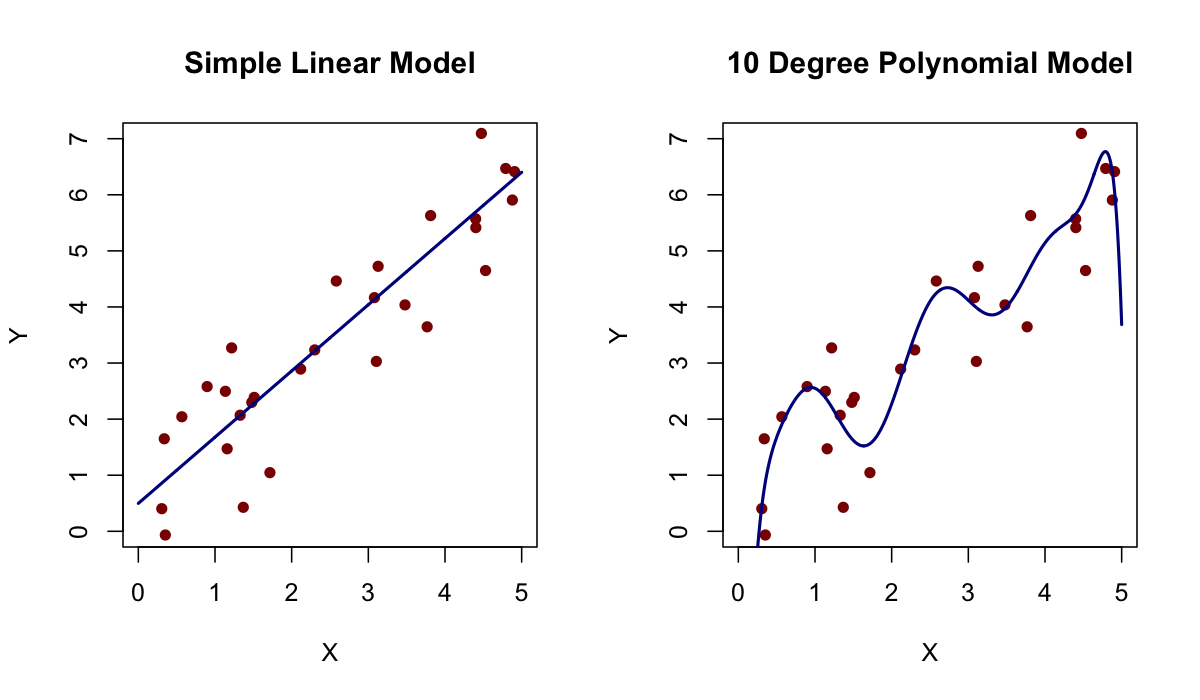
\includegraphics[width=0.75\linewidth]{overfit1.png}
	\end{figure}
	The polynomial model fits the initial data much better than the linear one.
	}
	\only<3>{
	\begin{figure}[htpb]
		\centering
		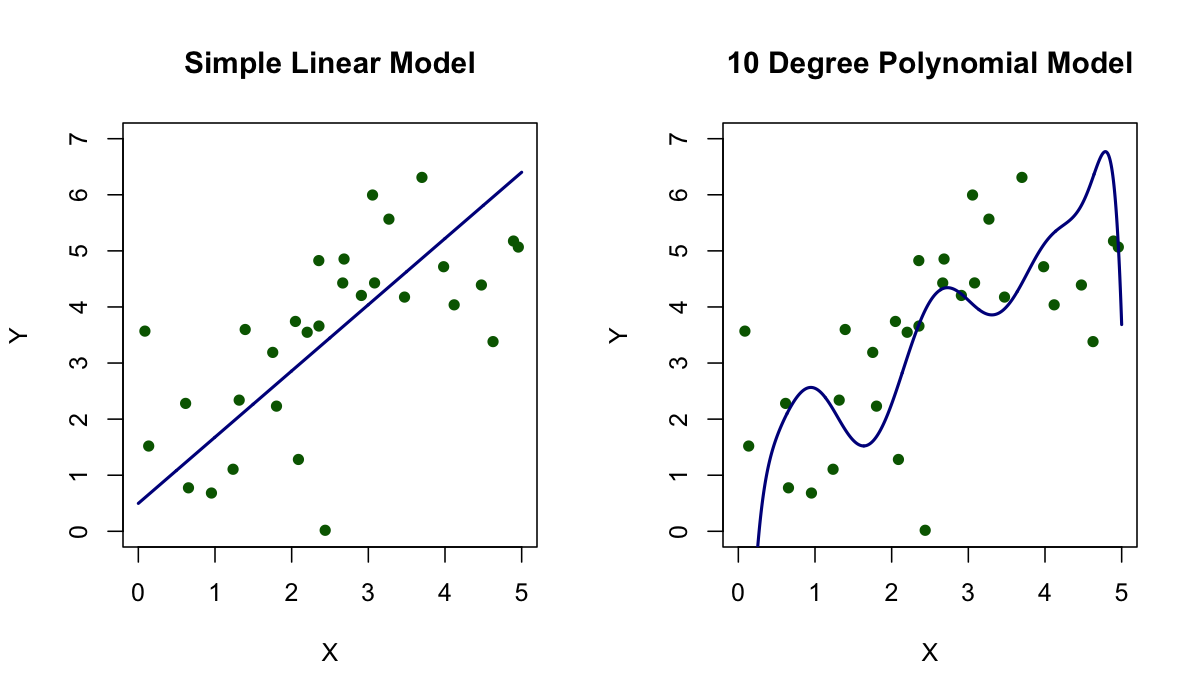
\includegraphics[width=0.75\linewidth]{overfit2.png}
	\end{figure}
	When taken to new data the polynomial model does much worse than the linear one.
	}
\end{frame}

\begin{frame}{Modeling Choices: Managing Model Complexity} 
	\label{frame:overfit2}
	How do we determine whether we are overfitting? A first guess might be to take the approach we took to model evaluation in Single Linear Regression and stop adding terms when our \(R^2\) falls. Just like in Single Linear Regression we can define 
	\[
		 R^2 = \frac{\text{SSR}}{\text{SST}} = 1 - \frac{\text{SSE}}{\text{SST}}  
	.\] 
	where as before \(\text{SSR} = \sum_{i=1}^n (\hat Y_i -  \bar Y)^2\), the sum of squares due to regression, \(\text{SST} = \sum_{i=1}^n (Y_i - \bar Y)^2\), the total sum of squares, and \(\text{SSE} = \sum_{i=1}^n \hat\eps_i^2\) is the sum of squared errors.
\end{frame}

\begin{frame}{Modeling Choices: Managing Model Complexity} 
	\label{frame:overfit3}
	\ucla{Problem:} The \(R^2\) will fall as long as we keep adding terms.

	\red{Why:} To see this let's use the representation \(R^2 = 1 - \frac{\text{SSE}}{\text{SST}}\). Across all models, \(\text{SST} = \sum_{i=1}^n (Y_i - \bar Y)^2\) will remain the same. However, the SSE will keep falling as we add more terms. 

\end{frame}

\begin{frame}{Modeling Choices: Managing Model Complexity} 
	\label{frame:overfit4}
	Why does the SSE fall as we add more terms? Note that we essentially choose our estimated parameters to minimize the SSE
	\begin{align*}
		\ucla{\hat\beta_0}, \ucla{\hat\beta_1} &= \arg\min_{b_0,b_1} \frac{1}{n}\sum_{i=1}^n (\underbrace{Y_i - b_0 - b_1X_{1,i}}_{\hat\eps_i})^2\\ 
		\ucla{\hat\beta_0},\ucla{\hat\beta_1},\ucla{\hat\beta_2} &= \arg\min_{b_0,b_1,b_2} \sum_{i=1}^n (\underbrace{Y_i - b_0 - b_1X_{1,i} - b_2 X_{2,i}}_{\hat\eps_i})^2
	\end{align*}
	\onslide<2->
	When using a third term, we could always recover the SSE from using two terms by keeping \(\ucla{\hat\beta_0}\) and \(\ucla{\hat\beta_1}\) the same and setting \( \ucla{\hat\beta_2} = 0\). The SSE mechanically must (weakly) fall when adding an additional term.

	\onslide<3->
	Since 
	\[
		R^2 = 1 - \frac{\text{SSE}}{\text{SST}} 
	,\] 
	this means that \(R^2\) also must fall as we add more terms.
\end{frame}

\begin{frame}{Modling Choices: Managing Model Complexity} 
	\label{frame:overfit5}
	For this reason, when evaluating multiple linear regression model we often use the \red{adjusted R-squared}. The adjusted \(R^2\) for a model with \(p\) terms and an intercept is given:
	\[
		\text{adj. } R^2 = 1 - \frac{\text{SSE}/(n-p-1)}{\text{SST}/(n-1)}  
	.\] 
	\green{Comments:}
	\begin{itemize}
		\item<2-> The adjusted \(R^2\) penalizes model complexity, it falls as  \(p\) increases.
		\item<3-> A first order approach to determining what model to use would be to add a potential (carefully thought through) term only if the adjusted \(R^2\) increases after adding the term.
		\begin{itemize}
			\item We will go over more formal approaches in the next lecture.
		\end{itemize}
		\item<4-> Adjusted \(R^2\) will be reported by most statistical software when running a multiple linear regression model.
	\end{itemize}
\end{frame}

\begin{frame}{Managing Model Complexity: Questions}
	\centering
	\red{\Large Questions?}
\end{frame} 


\end{document}


